
\section{개선}

\subsection{재귀함수 제거}

재귀 함수를 사용했을때에 loop문과 비교했을때 나타나는 문제점은 다음이 있다. 

\begin{itemize}
    \item 함수스택의 오버헤드
    \item 스택 오버플로우 위험성
    \item 메모리 부과    
\end{itemize}

그러나 quick sort의 반복문 사용은 복잡하며 코드가독성이 떨어진다.

\subsection{hybrid sort}

\subsubsection{Introsort}
Quicksort는 입력값에 대한 의존도가 크기에 일정 깊이로 들어같을 경우 이 밑을 heapsort로 처리하게 한다. heapsort는 Quicksort와 같은 시간복잡도가 $O(n \log n)$이지만 최선,최악에대해서 비교적 평균적인 수행시간을 보장한다. 일반적으로 한계 깊이를 $2\log_2 n$으로 설정하고있다.

\subsubsection{Quick insertion sort}
삽입 정렬(insertion sort)의 시간 복잡도는 $O(n^2)$이지만 베스트 케이스의 경우(완전히 정렬되있는경우) $O(n)$이다.(탐색만하고 넘어가기때문) 또한 작은 n에 대해서는 상대적으로 삽입정렬이 더 빠르게 되어 퀵소트 분할중 분할크기가 일정 n이하가 되면 삽입정렬으로 처리해 실제 quick sort를 사용했을때보다 시간적인 이득을 볼 수 있다. 또한 중복처리에 대해서 처리가 매우 빠르기 때문에 이에의한 성능향상도 생각해 볼 수 있다.
이 n은 일반적으로 10이며 이 값보다 작을때 선택정렬을 수행하도록한다. 

다음은 선택정렬을 수행하는 $n$에따른 수행시간이다. 여기서 테스트 케이스의 $N =10000$ 이다.

\begin{figure}[h!]
    \centering
    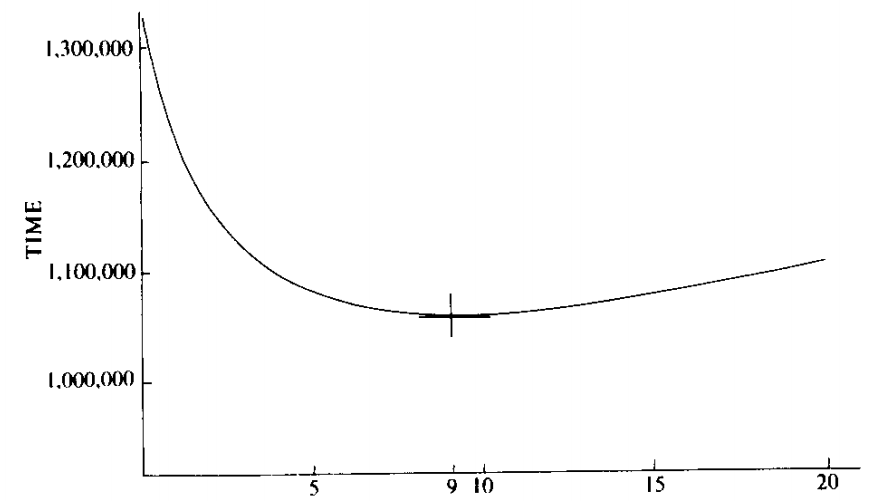
\includegraphics[scale=0.5]{{pic/q6.png}}
    \caption{삽입정렬 수행의 분할크기 n에 따른 퀵정렬 수행시간\cite{reference3}}
\end{figure}

\begin{lstlisting}[style = CStyle]
INSERTION_SORT(A)
    for j = 2 to A.length
        key = A[j]
        i = j - 1
        while i > 0 and A[i] > key
            A[i+1] = A[i]
            i = i-1
        A[i+1] = key
\end{lstlisting}

\subsection{중복값 처리}
네덜란드 국기 문제(Dutch national flag problem)로 다익스트라가 처음 제시한 이 문제는 quick sort의 중복값 입력에 대한 처리 문제를 다룬다. 배열에 같은 값으로만 들어왔을때를 생각해보자. 같은 값이 들어왔음에도 재귀는 $lg n$까지 깊이 들어간다. 이를 해결하기 위해 분할을 세 가지로한다.이를 3 way partitioning이라고한다. 기존의 왼쪽 오른쪽은 기존의 피봇값보다 \textbf{크고 작은}값이 들어가고 가운데에는 피봇과 같은 값을 모은다 그런후에 재귀의 범위를 왼쪽 오른쪽으로만 한다. 다음은 Dijstra가 제안한 해답이다. 코드는 c++로 작성되어 있다.
%\url{http://www.cs.princeton.edu/courses/archive/fall12/cos226/lectures/23Quicksort-2x2.pdf}
%https://www.cs.princeton.edu/~rs/talks/QuicksortIsOptimal.pdf

\begin{figure}[h!]
    \centering
    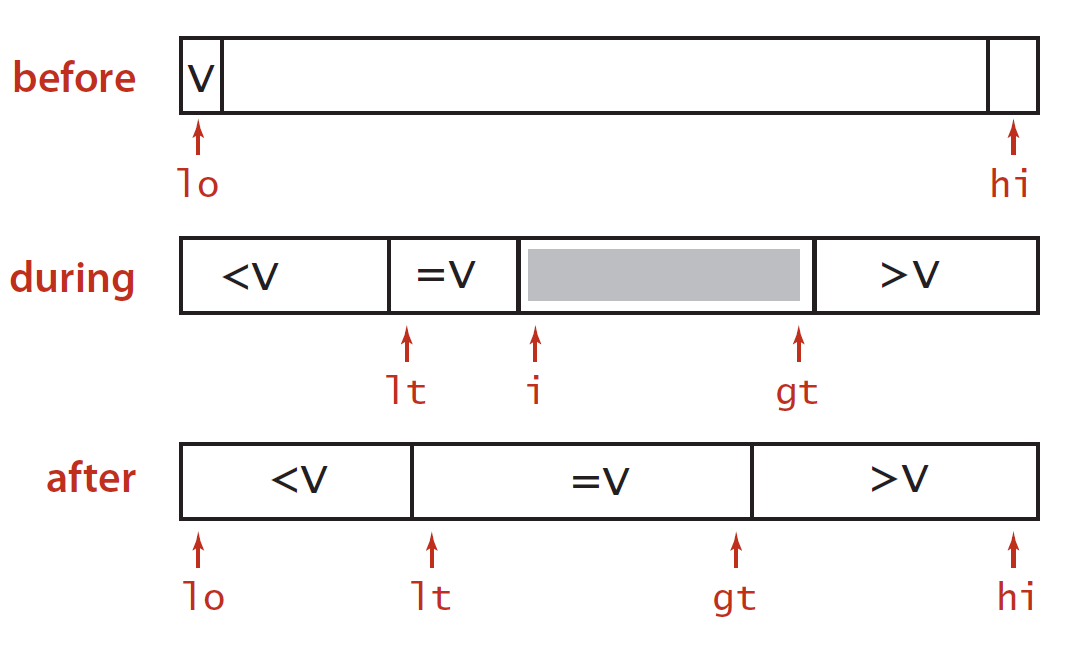
\includegraphics[scale=0.4]{{pic/q10.png}}
    \caption{3-way-partitioning 작동 방식 \cite{reference4}}
\end{figure}

\newpage


\begin{lstlisting}[style = CStyle]
void Quick3way(int a[], int lo, int hi)
{
    if (hi <= lo)
        return;
    int lt = lo, i = lo + 1, gt = hi;
    int v = a[lo];
    while (i <= gt)
    {
        if (a[i] < v)
        {
            std::swap(a[lt], a[i]);
            lt++, i++;
        }
        else if (a[i] > v)
        {
            std::swap(a[gt], a[i]);
            gt--;
        }
        else //a[i]==v
        {
            i++;
        }
    }
    Quick3way(a, lo, lt - 1);
    Quick3way(a, gt + 1, hi);
}
\end{lstlisting}

%\newpage

다음은 J. Bentley과 D. McIlroy 제안한 좀더 빠른 의사코드이다.

\begin{figure}[h!]
    \centering
    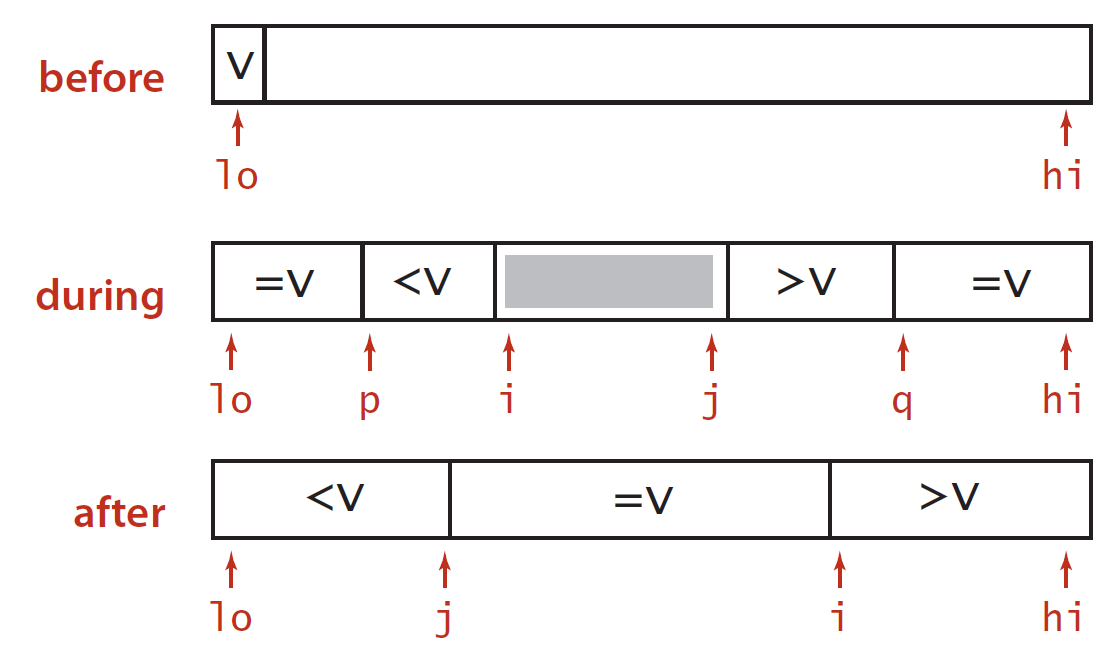
\includegraphics[scale=0.4]{{pic/q11.png}}
    \caption{Fast 3-way partitioning 작동 방식 \cite{reference4}}
\end{figure}

\begin{lstlisting}[style = CStyle]
    void quicksort(Item a[], int l, int r) 
    { 
        int i = l-1, j = r, p = l-1, q = r; Item v = a[r];
        if (r <= l) return;
        for (;;)
        {
            while (a[++i] < v) ;
            while (v < a[--j]) 
                if (j == l) break;
            if (i >= j) 
                break;
            exch(a[i], a[j]);
            if (a[i] == v) 
            {
                p++; 
                exch(a[p], a[i]); 
            }
            if (v == a[j]) 
            { 
                q--; 
                exch(a[j], a[q]); 
            }
        }
        exch(a[i], a[r]); 
        j = i-1; 
        i = i+1;
        for (k = l; k < p; k++, j--) 
            exch(a[k], a[j]);
        for (k = r-1; k > q; k--, i++) 
            exch(a[i], a[k]);
        quicksort(a, l, j);
        quicksort(a, i, r);
    }
    \end{lstlisting}

    

%http://penguin.ewu.edu/class/class/cscd300/Topic/AdvSorting/Sedgewick.pdf
\subsection{median of three}
Sedgewick이 제안했다. 위의 의사코드는 pivot값으로 맨끝의 값을 설정한다. 이는 역순정렬에 의한 최악의 케이스를 생성하기 때문에 이를 입력 p,r의 중점을 피봇값으로 설정하는것만으로도 상수시간에 개선가능하며, 이에 대한 응용으로 값을 랜덤으로 세개 뽑은후 중간값으로 하는 방법도 있다.

\subsection{Parallelization}
리커젼으로 나눠지는 두분할은 각각의 메모리 침범을 하지않는것이 명확하기 때문에 쓰레드 분할로 처리해도 문제가 없다. 이때의 가장 이상적인 수행시간은 트리 깊이인 $O(\lg n)$이다. 성능에 대해서는 병렬화의 고질적인 문제들도 복합적으로 고려해야한다.

 
and ...
멀티피봇에 대한 논의도 있으나 생략한다\footnote{다음이 좋은 참고 자료가 될것이다.\href{https://arxiv.org/abs/1905.00118}{Yukun Yao.(2019) A Detailed Analysis of Quicksort Algorithms with Experimental Mathematics} }. quicksort에 대한 연구는(특히 pivot설정) 매우 많이 진행되었고 진행되고있다.\footnote{원래 첫 제목은 All about Quicksort였으나 Quicksort에 대한 방대한 연구를 담아내기엔 상상이상으로 엄청난 논문이 줄을 이었다.}

